\chapter{Teoría del Algoritmo Genético aplicado a los horarios}

*** ESCRIBIR ACERCA DE LA TEORÍA DE AG ***

El algoritmo genético actualmente se utiliza para resolver problemas de optimización tanto discretos como continuos. Se basa en el mecanismo de la selección natural de Darwin, el cual nos indica que el individuo más apto sobrevive, por lo que entre mejores sean los padres, mejor es la descendencia.

Definimos a un cromosoma como una posible solución al problema. En nuestro caso representamos a un cromosoma por medio de una matriz con \textit{j\_materias} renglones y con 3 columnas las cuales representan la asignación de profesor, día y salón, respectivamente, por lo que el renglón $j$ indica que la materia $j$ es impartida por el profesor $i$, el día $t$, en el salón $k$.

El valor de adaptabilidad \textit{fit(x)}, de cada cromosoma, se asigna al evaluar su utilidad en la función objetivo, entre mejor sea el cromosoma, más alto será su valor de adaptabilidad. Los mejores cromosomas de la población actual pasan directamente a la siguiente generación. Se dice que la población evoluciona por medio de tres operadores hasta una condición de paro, los operadores son: \textit{selección, entrecruzamiento \textit{(crossover)} y mutación}.

Los pasos del algoritmo se muestran a continuación:


\begin{enumerate}
\item Se inicia con un grupo de cromosomas generados aleatoriamente, a los cuales se les calcula su valor de adaptabilidad

\item La probabilidad de que el cromosoma $k$ sea elegido para el entrecruzamiento \textit{(crossover)}, es:
  
\begin{equation*}
\begin{split}
&p_{k} = \dfrac{fit(x)}{\displaystyle \sum_{h = 1}^{pop} fit(h)} \,\,\,\, \text{ donde } pop \,\,\,\, \text{ es el tamaño de la población}\\
&\quad \text{ de cromosomas }
\end{split}
\end{equation*}


\item En el entrecruzamiento se mezclan dos padres para generar nuevas soluciones. Se genera un número aleatorio entre cero y uno, $r$, si $r < 0.6$  la primer columna de $M_{ij}$ y la primer columna de $M_{ti}$ del padre $1$ se copian en la nueva solución, las demás columnas se llenan con las columnas del padre $2$. Si la nueva solución no es factible, en la matriz $M_{ij}$, si alguna materia tiene asignada dos profesores, se selecciona uno de ellos de manera aleatoria y el otro se elimina de esa asignación; en caso de que alguna materia no tenga profesor asignado, se le asigna uno aleatoriamente.

\item Se actualiza la matriz $M_{ti}$.

\item Se aplica el operador \textit{mutación}, se selecciona un profesor de manera aleatoria y se cambia el día en el que más tiene clase por el día que menos clases imparte. Ésto se aplica para cada profesor de manera aleatoria, sin repetición.

\item Una vez generadas las nuevas soluciones se elige la mejor entre todas ellas.
\end{enumerate}

\section{Ciclo de la evolución natural}

\begin{figure}[H]
\centering
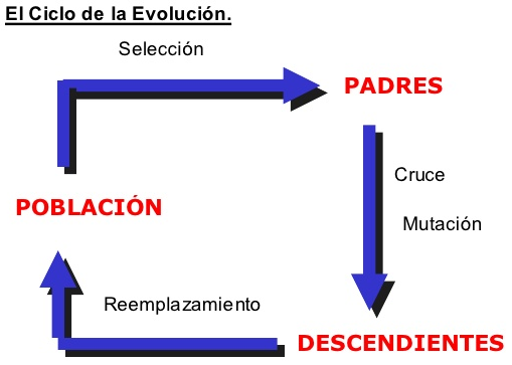
\includegraphics[scale = 0.45]{AG} %width=\textwidth
\caption{\textit{Algoritmo Genético}}
\end{figure}

\subsection{Selección}

\subsection{Cruce}

\subsection{Mutación}

\subsection{Reemplazamiento}


\section{Algoritmo Genético aplicado a la generación de asignaciones de grupos}


Matriz de 3 columnas (Materia-Horario-Profesor), la cual tiene la información de las asignaciones. A cada renglón de la matriz de esqueletos se agrega un profesor. Se genera con el esqueleto obtenido del proceso del AG y de las solicitudes de los profesores.



*** CAMBIAR \textit{esqueleto} POR \textit{asignación} ***
\begin{figure}[H]
\centering
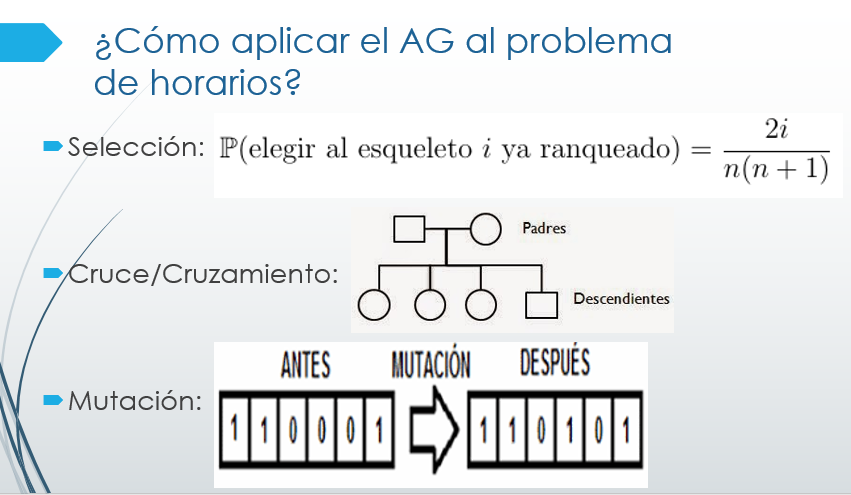
\includegraphics[scale = 0.45]{AG_aplicado} %width=\textwidth
\caption{\textit{Algoritmo Genético aplicado}}
\end{figure}


%\subsection{Calificación de asignaciones de grupo}
\subsection{Calificación de asignaciones}
%Los valores del modelo se muestran a continuación:
  
  %\begin{lstlisting}[language=R, caption= \textit{Método Holt-Winters aditivo}]
%Holt-Winters' additive method 
%
%Call:
% hw(y = tsData, h = 1, seasonal = "additive", level = c(q1, q2)) 
%
%  Smoothing parameters:
%    alpha = 0.1247 
%    beta  = 1 
%    gamma = 1 
%
%  Initial states:
%    l = 111 
%    b = -22.5 
%    s = -50 50
%
%  sigma:  155.8648
%\end{lstlisting}

%\begin{figure}[H]
%\centering
%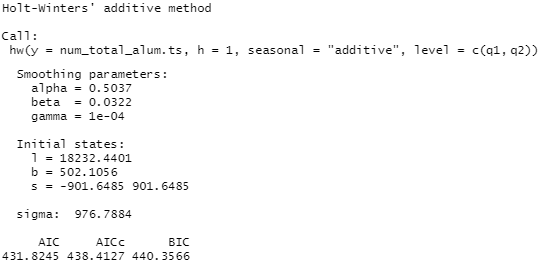
\includegraphics[scale = 0.8]{modelo_HW_total_alumnos_x_sem} %width=\textwidth
%\caption{\textit{Modelo del método aditivo de Holt-Winters: Total de alumnos por semestre}}
%\end{figure}
